\section{What Determines Teacher Distillability?}
\label{sec:distillability}

\subsection{Fixed-composition teacher-state intervention}
\label{sec:teacher-state}

To separate teacher state from composition, we compare jointly trained Teacher J with fusion-weight-only Teacher A at the same $\alpha=0.5$. Their teacher validation-subset NLLs are 4.300644 and 6.376220. Teacher J produces positive transfer in all three students, whereas Teacher A produces negative transfer in all three: mean gains are $+0.155665\pm0.007692$ and $-0.027654\pm0.006822$ (Table~\ref{tab:teacher_state}). The paired state contrast is
\begin{equation}
Q=\mathrm{NLL}_{\mathrm{KD,A}}-\mathrm{NLL}_{\mathrm{KD,J}}
=+0.183319\pm0.001375,
\label{eq:teacher-state-contrast}
\end{equation}
with all three differences positive.

The reversal shows that teacher training state matters even with fixed architecture and fusion composition. It does not isolate scalar likelihood as the cause: joint training also changes branch representations and the distribution of errors. Better predictive quality accompanies more useful supervision here, but the intervention is on trained teacher state, not NLL alone. Optimization gates and the documented protocol amendment are retained in Appendix~\ref{app:protocols}.

\subsection{A globally weaker teacher can still help}
\label{sec:weaker-teacher}

The Grassmann-only source supplies a counterexample to a simple likelihood rule. Its validation-subset NLL is 4.652064, worse than every matched CE endpoint on that subset, yet its test gain is positive in all three students, averaging $+0.040991\pm0.006733$ (Table~\ref{tab:weaker_teacher}). A globally weaker teacher can therefore provide useful supervision under this continuation protocol.

The reference student is the validation-selected CE continuation, not an arbitrary initialization. Teacher residual advantage and transfer gain also use different held-out scopes, as stated in the table. This result does not make teacher quality irrelevant; together with the state reversal, it shows that global held-out teacher likelihood alone is insufficient to determine distillability. Figure~\ref{fig:teacher_quality} summarizes these complementary controls without assigning a geometric cause to the gain.

% Numeric rows formatted from frozen archived tables; caption revised 2026-10-08.
\begin{table}[htbp]
\centering\small
\begin{tabular}{lrrrr}
\toprule
Teacher/state contrast & Teacher val NLL & Gain/contrast & Sample SD & Signs \\
\midrule
Joint J & 4.300644 & 0.155665 & 0.007692 & 3/3 + \\
Alpha-only A & 6.376220 & -0.027654 & 0.006822 & 3/3 -- \\
$Q$ (student test contrast) & -- & 0.183319 & 0.001375 & 3/3 + \\
\bottomrule
\end{tabular}
\caption{Fixed-composition teacher-state intervention on WikiText-2. Teacher NLL uses the same 512-chunk validation subset; gains are CE-relative test endpoints over three students. $Q$ compares A with J within a student. Composition is fixed, but trained representations differ.}
\label{tab:teacher_state}
\end{table}

% Generated from frozen sources by build_tables.py; not a prose draft.
\begin{table}[htbp]
\centering\small
\begin{tabular}{lrr}
\toprule
Seed & Teacher residual vs C0 & KD test gain \\
\midrule
42 & -0.266520 & 0.046771 \\
123 & -0.253492 & 0.033598 \\
456 & -0.251006 & 0.042604 \\
\bottomrule
\end{tabular}
\caption{A globally weaker teacher can still transfer positively (planning table).}
\label{tab:weaker_teacher}
\par\smallskip\begin{minipage}{0.96\linewidth}\footnotesize Residual is C0 validation-subset NLL minus teacher NLL. All residuals are negative while gains are positive. This refutes a universal necessity rule; it does not show that weak teachers are usually better or that likelihood is irrelevant.\end{minipage}
\end{table}

\begin{figure}[htbp]
\centering
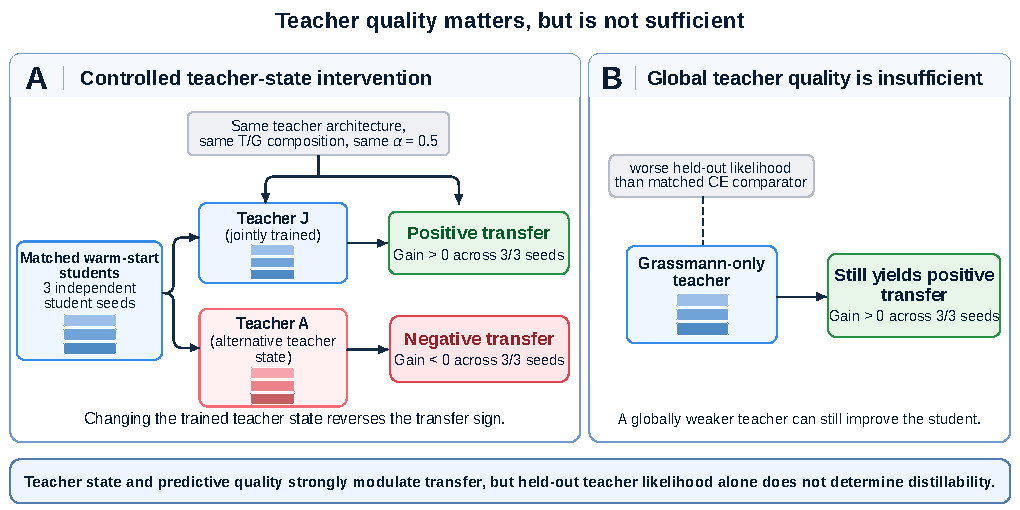
\includegraphics[width=\linewidth]{figures/fig3_teacher_quality.pdf}
\caption{Teacher-state and likelihood controls on WikiText-2. Changing trained teacher state reverses transfer at fixed composition. A weaker Grassmann-only source still transfers positively. Neither control establishes scalar-likelihood causality or a geometry-specific KD advantage.}
\label{fig:teacher_quality}
\end{figure}
